\documentclass[fleqn]{article}
\usepackage[nodisplayskipstretch]{setspace}
\usepackage{amsmath, nccmath}
\usepackage{amssymb}
\usepackage{enumitem}
\usepackage{etoolbox}
\usepackage{graphicx}
\usepackage{float}
\usepackage{changepage}
\usepackage{environ,capt-of}
\usepackage{matlab-prettifier}

\newcommand{\zerodisplayskip}{
	\setlength{\abovedisplayskip}{0pt}%
	\setlength{\belowdisplayskip}{0pt}%
	\setlength{\abovedisplayshortskip}{0pt}%
	\setlength{\belowdisplayshortskip}{0pt}%
	\setlength{\mathindent}{0pt}}

\makeatletter
	\newenvironment{equationCenter}{\@fleqnfalse\begin{equation*}}{\end{equation*}}
\makeatother

\let\oldfigure\figure% Store original figure float environment
\let\endoldfigure\endfigure
\RenewEnviron{figure}[1][H]{% Update figure environment
  %\par\vspace{\intextsep}% Assume in-text placement, so insert appropriate vertical spacing
  \noindent
  % \patchcmd{<cmd>}{<search>}{<replace>}{<success>}{<failure>}
  \patchcmd{\BODY}{\caption}{\captionof{figure}}{}{}% Replace \caption with \captionof{figure} inside \BODY
  % Set "figure"
  \begin{minipage}{\linewidth}
    \BODY
  \end{minipage}
  %\par\vspace{\intextsep}% Assume in-text placement, so insert appropriate vertical spacing
}

\title{Homework 4}
\author{Owen Sowatzke}
\date{October 16, 2023}

\begin{document}
	\offinterlineskip
	\setlength{\lineskip}{12pt}
	\zerodisplayskip
	\maketitle
	
	\begin{enumerate}[nolistsep]
		\item Define $T \in \mathcal{L}(\mathbb{F}^2)$ by
		
			\begin{equationCenter}
				T(w,z) = (z,w)
			\end{equationCenter}
			
			Find all eigenvalues and eigenvectors of $T$.
	
			$Tv = {\lambda}v$
			%
			$\Rightarrow T(w,z) = \lambda(w,z)$
			%
			$\Rightarrow(z,w) = \lambda(w,z)$
			%
			$\Rightarrow(z,w) = ({\lambda}w,{\lambda}z)$
			
			$z = {\lambda}w$
			%
			$\Rightarrow w = \lambda({\lambda}w)$
			%
			$\Rightarrow w = {\lambda}^2 w$
			%
			$\Rightarrow {\lambda}^2 = 1$
			%
			$\Rightarrow \lambda = \pm \sqrt{1}$
			%
			$\Rightarrow \lambda = \pm 1$
			
			$\therefore \lambda_1 = 1,\ \lambda_2 = -1$
			
			$\lambda_1 = 1 \Rightarrow z = w \Rightarrow v_1 = (w, w)$
			
			$\lambda_2 = -1 \Rightarrow z = -w \Rightarrow v_2 = (w, -w)$
			
		\item Suppose $T \in \mathcal{L}(V)$ and $\text{dim range}\ T = k$. Prove that $T$ has at most $k + 1$ distinct eigenvalues.
	
			Let $v_j$ be an eigenvector of $T$. Then, $Tv_j = {\lambda_j}v_j$.
			
			Consider $\lambda_j \neq 0$:
			
			\begin{equation*}
				\Rightarrow \frac{1}{\lambda_j}T(v_j) = v_j \Rightarrow T\left(\frac{v_j}{\lambda_j}\right) = v_j	 \Rightarrow v_j \in \mathcal{R}(T)			
			\end{equation*}
			
			There are at most $k$ linearly independent eigenvectors $v_j$ that satisfy this expression. The eigenvalues corresponding to linearly independent eigenvectors are distinct.
			
			$\therefore$ there can be at most $k$ distinct nonzero eigenvalues $\lambda_j$.
			
			\pagebreak
			Consider $\lambda_j = 0$:
			
			For $\lambda_j=0$, there must be a nonzero eigenvector $v_j$ such that
			
			$Tv_j = 0 \Rightarrow v_j \in n(T)$
			
			Let $n(T) \neq \{0\} \Rightarrow \exists\ v_j \neq 0$ such that $Tv_j = 0$
			
			For this case, there is an eigenvalue $\lambda_j = 0$.
			
			$\therefore$ there are at most $k + 1$ distinct eigenvalues.
		
		\item \textbf{Electrical Oscillators:} Consider the electric circuit shown below.
		
			{\centering
				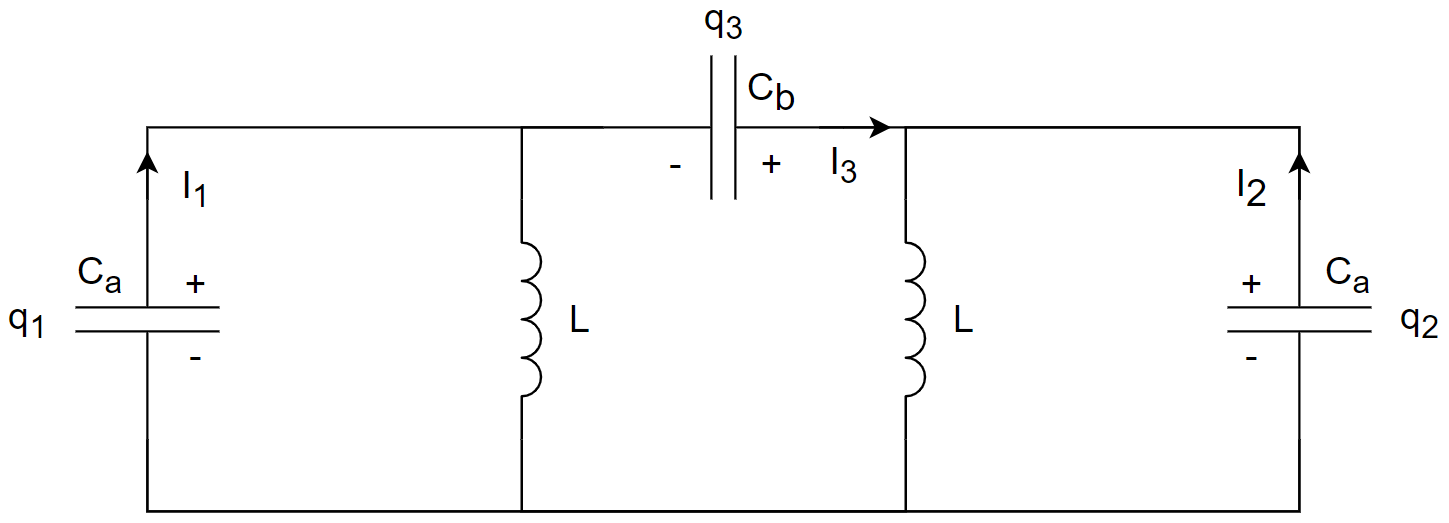
\includegraphics[width=0.75\textwidth]{Homework4_Circuit_Sowatzke.png}
			\par}
			
			Three capacitors (two with capacitance $C_a$ and one with capacitance $C_b$) are charged with (potentially different) charges $q_1$, $q_2$, and $q_3$ and connected with the polarity shown to two inductors of inductance $L$.
			
			In this problem we will explore how to convert the physical properties of this system into a linear map and how, with a strategic choice, we can convert the general linear map into an \textit{eigenvalue equation} that describes the system. In future homework problems, we will work on solving the \textit{eigenvalue equation} to determine the \textit{natural modes} of the system
			
			\begin{enumerate}[nolistsep]
				\item Remembering that the voltage difference across a capacitor and inductor can be written as $V=q/C$ and $V=L(dI/dt)$, respectively ($I$ is the \textit{net} current through the inductor), derive two equations that relate the charges $q_1$ and $q_2$ to the loop currents $I_1$, $I_2$, and $I_3$.
				
					\pagebreak
					\begin{equation*}
						\frac{q_1}{C_a} = L\frac{d}{dt}(I_1 - I_3)\Rightarrow q_1 = LC_a\frac{d}{dt}(I_1 - I_3)
					\end{equation*}
					%
					\begin{equation*}
						\frac{q_2}{C_a} = L\frac{d}{dt}(I_2 + I_3) \Rightarrow q_2 = LC_a\frac{d}{dt}(I_2 + I_3)
					\end{equation*}
				
				\item Remember that $I=dq/dt=\dot{q}$ and rewrite the equations so that they now relate $q_1$ and $q_2$ to $\ddot{q_1}$, $\ddot{q_2}$, and $\ddot{q_3}$.
				
					$q_1 = LC_a(\ddot{q_1} - \ddot{q_3})$
					
					$q_2 = LC_a(\ddot{q_2} + \ddot{q_3})$
					
				\item Using $V=q/C$, derive a relationship between $q_1$, $q_2$, and $q_3$. Take multiple time derivatives to convert this into a relationship between $\ddot{q_1}$, $\ddot{q_2}$, and $\ddot{q_3}$. Use this result to eliminate $\ddot{q_3}$ from your expressions for $q_1$ and $q_2$.
				
					\begin{equation*}
						\frac{q_1}{C_a} + \frac{q_3}{C_b} = \frac{q_2}{C_a} \Rightarrow \frac{\ddot{q_1}}{C_a} + \frac{\ddot{q_3}}{C_b} = \frac{\ddot{q_2}}{C_a}
					\end{equation*}
					%
					\begin{equation*}
						 \Rightarrow \frac{\ddot{q_3}}{C_b} = \frac{\ddot{q_2}}{C_a} - \frac{\ddot{q_1}}{C_a} \Rightarrow \ddot{q_3} = \frac{C_b}{C_a}(\ddot{q_2} - \ddot{q_1})
					\end{equation*}
					%
					\begin{equation*}
						q_1 = LC_a\left(\ddot{q_1} - \frac{C_b}{C_a}(\ddot{q_2} - \ddot{q_1})\right) \Rightarrow q_1 = LC_a\ddot{q_1} - LC_b(\ddot{q_2} - \ddot{q_1})
					\end{equation*}
					%
					$\Rightarrow q_1 = LC_a\ddot{q_1} - LC_b\ddot{q_2} + LC_b\ddot{q_1} \Rightarrow q_1 = L(C_a + C_b)\ddot{q_1} - LC_b\ddot{q_2}$
					
					\begin{equation*}
						q_2 = LC_a\left(\ddot{q_2} + \frac{C_b}{C_a}(\ddot{q_2} - \ddot{q_1})\right) \Rightarrow q_2 = LC_a\ddot{q_2} + LC_b(\ddot{q_2} - \ddot{q_1})
					\end{equation*}
					%
					$\Rightarrow q_2 = LC_a\ddot{q_2} + LC_b\ddot{q_2} - LC_b\ddot{q_1} \Rightarrow q_2 = - LC_b\ddot{q_1} + L(C_a + C_b)\ddot{q_2}$
					
				\item Algebraically rearrange these equations into the following matrix form:
				
					\begin{equationCenter}
						\begin{bmatrix}\ddot{q_1} \\ \ddot{q_2}\end{bmatrix} = M \begin{bmatrix}q_1 \\ q_2\end{bmatrix}
					\end{equationCenter}
					
					where $M$ is a $2 \times 2$ matrix.
					
					\pagebreak
					\begin{equation*}
						q_1 = L(C_a + C_b)\ddot{q_1} - LC_b\ddot{q_2} \Rightarrow LC_b\ddot{q_2} = L(C_a + C_b)\ddot{q_1} - q_1
					\end{equation*}
					%
					\begin{equation*}
						\Rightarrow \ddot{q_2} = \frac{C_a + C_b}{C_b}\ddot{q_1} - \frac{1}{LC_b}q_1
					\end{equation*}
					%
					\begin{equation*}
						q_2 = - LC_b\ddot{q_1} + L(C_a + C_b)\ddot{q_2}
					\end{equation*}
					%
					\begin{equation*}
						\Rightarrow q_2 = - LC_b\ddot{q_1} + L(C_a + C_b)\left(\frac{C_a + C_b}{C_b}\ddot{q_1} - \frac{1}{LC_b}q_1\right)
					\end{equation*}
					%
					\begin{equation*}
						\Rightarrow q_2 = - LC_b\ddot{q_1} + \frac{L(C_a + C_b)^2}{C_b}\ddot{q_1} - \frac{C_a + C_b}{C_b}q_1
					\end{equation*}
					%
					\begin{equation*}
						\Rightarrow q_2 = - LC_b\ddot{q_1} + \frac{L(C_a^2 + 2C_aC_b + C_b^2)}{C_b}\ddot{q_1} - \frac{C_a + C_b}{C_b}q_1
					\end{equation*}
					%
					\begin{equation*}
						\Rightarrow q_2 = \frac{L(C_a^2 + 2C_aC_b + C_b^2) - LC_b^2}{C_b}\ddot{q_1} - \frac{C_a + C_b}{C_b}q_1
					\end{equation*}
					%
					\begin{equation*}
						\Rightarrow q_2 = \frac{L(C_a^2 + 2C_aC_b)}{C_b}\ddot{q_1} - \frac{C_a + C_b}{C_b}q_1
					\end{equation*}
					%
					\begin{equation*}
						\Rightarrow q_2 = \frac{LC_a(C_a + 2C_b)}{C_b}\ddot{q_1} - \frac{C_a + C_b}{C_b}q_1
					\end{equation*}
					%
					\begin{equation*}
						\Rightarrow \frac{LC_a(C_a + 2C_b)}{C_b}\ddot{q_1} = \frac{C_a + C_b}{C_b}q_1 + q_2
					\end{equation*}
					%
					\begin{equation*}
						\Rightarrow \ddot{q_1} = \frac{C_a + C_b}{LC_a(C_a + 2C_b)}q_1 + \frac{C_b}{LC_a(C_a + 2C_b)}q_2
					\end{equation*}
					%
					\begin{equation*}
						\ddot{q_2} = \frac{C_a + C_b}{C_b}\ddot{q_1} - \frac{1}{LC_b}q_1
					\end{equation*}
					%
					\begin{equation*}
						\Rightarrow \ddot{q_2} = \frac{C_a + C_b}{C_b}\left(\frac{C_a + C_b}{LC_a(C_a + 2C_b)}q_1 + \frac{C_b}{LC_a(C_a + 2C_b)}q_2\right) - \frac{1}{LC_b}q_1
					\end{equation*}
					%
					\begin{equation*}
						\Rightarrow \ddot{q_2} = \frac{(C_a + C_b)^2}{LC_aC_b(C_a + 2C_b)}q_1 + \frac{C_a + C_b}{LC_a(C_a + 2C_b)}q_2 - \frac{1}{LC_b}q_1
					\end{equation*}
					%
					\begin{equation*}
						\Rightarrow \ddot{q_2} = \frac{(C_a + C_b)^2 - C_a(C_a + 2C_b)}{LC_aC_b(C_a + 2C_b)}q_1 + \frac{C_a + C_b}{LC_a(C_a + 2C_b)}q_2
					\end{equation*}
					%
					\begin{equation*}
						\Rightarrow \ddot{q_2} = \frac{C_a^2 + 2C_aC_b + C_b^2 - C_a^2 - 2C_aC_b}{LC_aC_b(C_a + 2C_b)}q_1 + \frac{C_a + C_b}{LC_a(C_a + 2C_b)}q_2
					\end{equation*}
					%
					\begin{equation*}
						\Rightarrow \ddot{q_2} = \frac{C_b^2}{LC_aC_b(C_a + 2C_b)}q_1 + \frac{C_a + C_b}{LC_a(C_a + 2C_b)}q_2
					\end{equation*}
					%
					\begin{equation*}
						\Rightarrow \ddot{q_2} = \frac{C_b}{LC_a(C_a + 2C_b)}q_1 + \frac{C_a + C_b}{LC_a(C_a + 2C_b)}q_2
					\end{equation*}
					%
					$\therefore$ we can express the equations in the following form:
					\begin{equation*}
						\begin{bmatrix}\ddot{q_1} \\ \ddot{q_2}\end{bmatrix} = M \begin{bmatrix}q_1 \\ q_2\end{bmatrix}
					\end{equation*}
					
					where:
					
					\begin{equation*}
						M = \begin{bmatrix}
							\frac{C_a + C_b}{LC_a(C_a + 2C_b)} &  \frac{C_b}{LC_a(C_a + 2C_b)} \\
							\frac{C_b}{LC_a(C_a + 2C_b)} & \frac{C_a + C_b}{LC_a(C_a + 2C_b)}
						\end{bmatrix}
					\end{equation*}
				\item Show that $M$ is a linear map from $\mathbb{R}^2 \rightarrow \mathbb{R}^2$.
				
					$M$ maps $\begin{bmatrix}q_1 \\ q_2 \end{bmatrix} \in \mathbb{R}^2$ to $\begin{bmatrix}\ddot{q_1} \\ \ddot{q_2} \end{bmatrix} \in \mathbb{R}^2$.
					
					$\therefore$ $M$ is a map from $\mathbb{R}^2 \rightarrow \mathbb{R}^2$.
					
					For $M$ to be a linear map, it must satisfy additivity and homogeneity.
					
					Rewrite $M$ as follows:
					
					\begin{equation*}
						M = \begin{bmatrix}
							A_{11} & A_{12} \\ A_{21} & A_{22}
						\end{bmatrix}
					\end{equation*}
					
					Check whether $M$ satisfies additivity:
					
					Let $v = \begin{bmatrix}q_1 \\ q_2\end{bmatrix} \in \mathbb{R}^2$ and $\bar{v} = \begin{bmatrix}\bar{q}_1 \\ \bar{q}_2\end{bmatrix} \in \mathbb{R}^2$
					
					\begin{equation*}
						M(v + \bar{v}) = \begin{bmatrix} A_{11} & A_{12} \\ A_{21} & A_{22}\end{bmatrix}\begin{bmatrix} q_1 + \bar{q}_1 \\ q_2 + \bar{q}_2 \end{bmatrix} = \begin{bmatrix} A_{11}(q_1 + \bar{q}_1) + A_{12}(q_2 + \bar{q}_2) \\ A_{21}(q_1 + \bar{q}_1) + A_{22}(q_2 + \bar{q}_2) \end{bmatrix}
					\end{equation*}
					%
					\begin{equation*}
						= \begin{bmatrix}(A_{11}q_1 + A_{12}q_2) + (A_{11}\bar{q}_1 + A_{12}\bar{q}_2) \\ (A_{21}q_1 + A_{22}q_2) + (A_{21}\bar{q}_1 + A_{22}\bar{q}_2)\end{bmatrix}
					\end{equation*}
					%
					\begin{equation*}
						= \begin{bmatrix}A_{11}q_1 + A_{12}q_2 \\ A_{21}q_1 + A_{22}q_2 \end{bmatrix} + \begin{bmatrix}A_{11}\bar{q}_1 + A_{12}\bar{q}_2 \\ A_{21}\bar{q}_1 + A_{22}\bar{q}_2 \end{bmatrix}
					\end{equation*}
					%
					\begin{equation*}
						= \begin{bmatrix}A_{11} & A_{12} \\ A_{21} & A_{22}\end{bmatrix}\begin{bmatrix}q_1 \\ q_2\end{bmatrix} +  \begin{bmatrix}A_{11} & A_{12} \\ A_{21} & A_{22}\end{bmatrix}\begin{bmatrix}\bar{q}_1 \\ \bar{q}_2\end{bmatrix} = Mv + M\bar{v}
					\end{equation*}
					%
					$\Rightarrow$ $M$ satisfies additivity.
					
					Check whether $M$ satisifies homogeneity:
					
					Let $v = \begin{bmatrix}q_1 \\ q_2\end{bmatrix} \in \mathbb{R}^2$ and $\lambda \in \mathbb{R}$.
					
					\begin{equation*}
						M({\lambda}v) = \begin{bmatrix} A_{11} & A_{12} \\ A_{21} & A_{22}\end{bmatrix}\begin{bmatrix} {\lambda}q_1 \\ {\lambda}q_2\end{bmatrix} = \begin{bmatrix} A_{11}({\lambda}q_1) + A_{12}({\lambda}q_2) \\ A_{21}({\lambda}q_1) + A_{22}({\lambda}q_2) \end{bmatrix}
					\end{equation*}
					%					
					\begin{equation*}
						= \begin{bmatrix} {\lambda}A_{11}q_1 + {\lambda}A_{12}q_2 \\ {\lambda}A_{21}q_1 + {\lambda}A_{22}q_2 \end{bmatrix} = \begin{bmatrix} \lambda(A_{11}q_1 + A_{12}q_2)\\ \lambda(A_{21}q_1 + A_{22}q_2)\end{bmatrix} = \lambda\begin{bmatrix}A_{11}q_1 + A_{12}q_2 \\ A_{21}q_1 + A_{22}q_2\end{bmatrix}
					\end{equation*}
					%
					\begin{equation*}
						= \lambda\begin{bmatrix}A_{11} & A_{12}\\ A_{21} & A_{22}\end{bmatrix}\begin{bmatrix}q_1 \\ q_2\end{bmatrix} = {\lambda}Mv
					\end{equation*}
					%
					$\Rightarrow$ $M$ satisfies homogeneity.
					
					Because $M$ satisifies both additivity and homogeneity, it is a linear map from $\mathbb{R}^2 \rightarrow \mathbb{R}^2$
					
				\item To proceed, we make the \textit{Anastz} (a fancy German word that roughly means "guess solution") that $q_1$ and $q_2$, will have a time-dependence that is \textit{harmonic} (sinusoidal). Let $q_1 = A_1e^{j{\omega}t}$ and $q_1 = A_2e^{j{\omega}t}$. Substitute these values into your matrix equation, take the derivatives, and simplify. Your result should involve the vector $(A_1, A_2)$ on both sides of the equation. Note that the form of your result is now a standard eigenvalue equation.
				
				\begin{equation*}
					\begin{bmatrix}\ddot{q_1} \\ \ddot{q_2}\end{bmatrix} = M\begin{bmatrix}q_1 \\ q_2\end{bmatrix}
				\end{equation*}
				
				Let $q_1 = A_1e^{j{\omega}t}$ and $q_1 = A_2e^{j{\omega}t}$:
				
				\begin{equation*}
					\Rightarrow \begin{bmatrix}A_1(j\omega)^2e^{j{\omega}t} \\ A_2(j\omega)^2e^{j{\omega}t}\end{bmatrix} = M\begin{bmatrix}A_1e^{j{\omega}t} \\ A_2e^{j{\omega}t}\end{bmatrix}
				\end{equation*}
				%
				\begin{equation*}
					\Rightarrow - {\omega}^2\begin{bmatrix} A_1e^{j{\omega}t} \\ A_2e^{j{\omega}t}\end{bmatrix} = M\begin{bmatrix}A_1e^{j{\omega}t} \\ A_2e^{j{\omega}t}\end{bmatrix}
				\end{equation*}
				%
				\newpage
				Because $e^{j{\omega}t}$ is common to all terms, we can remove it from the equation.
				
				\begin{equation*}
					\Rightarrow - {\omega}^2\begin{bmatrix} A_1 \\ A_2\end{bmatrix} = M\begin{bmatrix}A_1 \\ A_2\end{bmatrix}
				\end{equation*}
				
				Let $\lambda = -{\omega}^2$ and $v = \begin{bmatrix} A_1 \\ A_2 \end{bmatrix}$
				
				$\Rightarrow {\lambda}v = Mv$ (the standard eigenvalue equation)
			\end{enumerate}
		\item \textbf{Repeated Application of Linear Map:} Consider the linear map $T$: $\mathbf{R}^5 \rightarrow \mathbf{R}^5$ represented in matrix form on the standard basis as
		
			\begin{equationCenter}
				M[T] = \begin{bmatrix}
					1 &  0 & -1 &  1 &  1\\
					0 &  1 &  0 &  0 &  1\\
				   -1 &  0 & -1 & -1 & -1\\
				    1 &  0 & -1 &  0 &  1\\
				    1 &  1 & -1 &  1 & -1
				\end{bmatrix}
			\end{equationCenter}
			
			This problem will investigate what happens when a linear map (in this case T) is repeatedly applied to a vector.
			
			\textbf{Important Note:} the map T, like most maps, does not maintain the length of a vector. Repeated application can result in very large (or very small) values for some of the coordinates. To avoid complications introduced by this effect, we will be frequently \textit{normalizing} the vectors as we proceed. For the purposes of this exercise, \textit{normalizing a vector} is defined as dividing the vector by the vector element with the largest \textit{absolute value}. That is, the vector is scaled by an amount that turns the element with the largest absolute value into the value 1.
			
			\begin{enumerate}
				\item Write a MATLAB script that does the following:
					\begin{itemize}
						\item Generate a random vector, v, in $\mathbb{R}^5$ and normalize it. Feel free to constrain your random number selection to the default domain of the \textbf{rand} command.
						
						\item Apply the map T to the normalized input vector. Normalize and store the result. Now apply the map T to this normalized output vector. Normalize and store the result. Repeat in this manner until you have generated the output for 1-25 repeated applications of T to a given random initial vector.
					\end{itemize}
					
				\item Make a plot that compares the results for 1, 3, 5, 10, and 25 applications of T to a given random initial vector. Comment on the results.
				
					\begin{figure}[H]				
							\centerline{\fbox{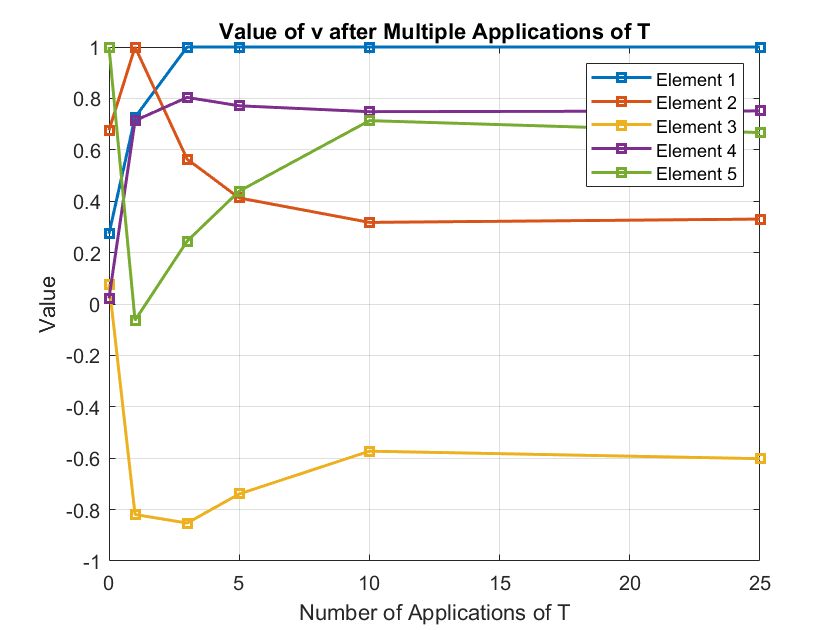
\includegraphics[width=0.5\textwidth]{multiple_apps_of_T.png}}}
							\caption{Value of v after Multiple Applications of T.}
							\label{multiple_apps_of_T}
					\end{figure}
				
					After multiple applications of T, the random vector converges to a stable result.
					
					%The random vector can be written as a linear combination of the eigenvectors. After multiple applications of T, v converges to the eigenvector corresponding to the largest eigenvalue. The eigenvector components corresponding to the smaller eigenvalues are exponentially reduced in size by each application of T.
					
				\item Make a plot that compares the results from 25 applications of T to 5 different random initial vectors. Comment on the results.
				
					\begin{figure}[H]				
							\centerline{\fbox{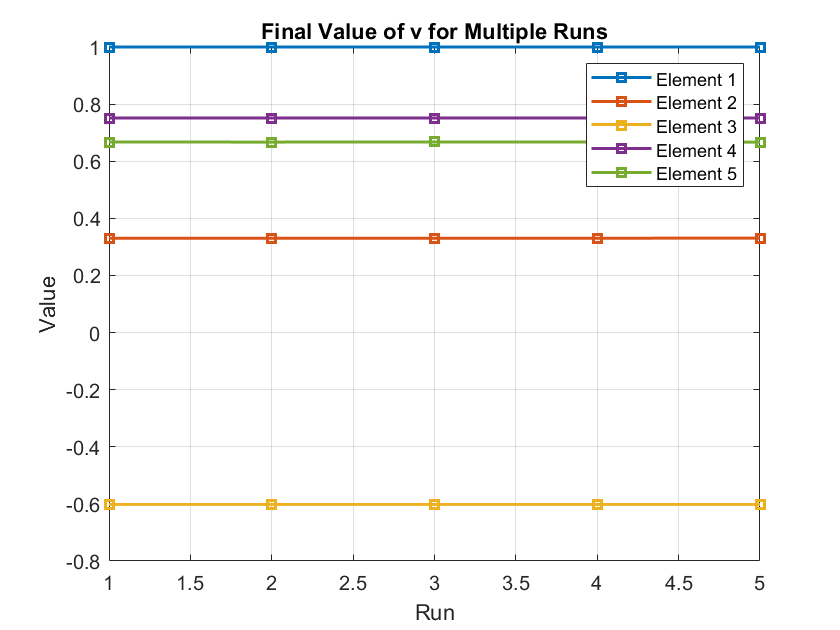
\includegraphics[width=0.5\textwidth]{final_value_multiple_runs.png}}}
							\caption{Final Value of v for Multiple Runs.}
							\label{final_value_multiple_runs}
					\end{figure}
					
					The final value of v is the same for each run (i.e. the starting value of v does not influence the result).
					
				\item In class, we are just starting to learn how to find eigenvectors and eigenvalues of a linear map. However, for this exercise, we will allow you to use the numerical routine in MATLAB. The form of the command in [V,D] = eig(T). The routine will return two matrices. V is a matrix whose column whose columns are the eigenvectors of T, and D is a diagonal matrix whose values are the corresponding eigenvalues, i.e., the eigenvalue in column n is associated with the eigenvector in column n. Modify your script to find the eigenvalues and eigenvectors of T. Locate the eigenvalue with the largest absolute value and call its corresponding eigenvector w. Normalize w.
				
				\item Make a plot that compares the normalized version of w to your results for 1, 5, and 10 applications of T to a given random initial vector. Comment on the results and argue intuitively about how they are related to the concept of an invariant subspace.
				
					\begin{figure}[H]				
							\centerline{\fbox{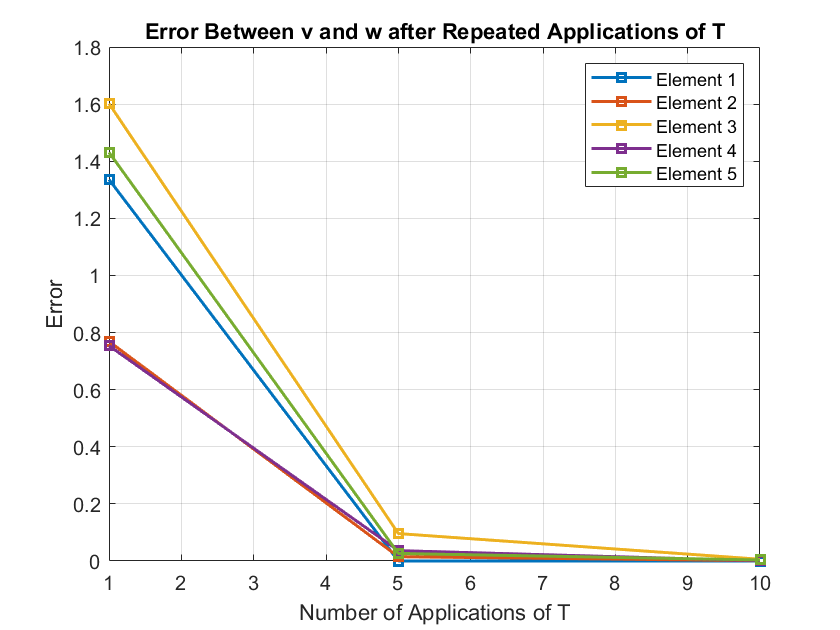
\includegraphics[width=0.5\textwidth]{comparison_to_eigenvalue.png}}}
							\caption{Error Between v and w after Repeated Applications of T.}
							\label{comparison_to_eigenvalue}
					\end{figure}
				
					The random input vector converges to w (the eigenvector corresponding to the largest eigenvalue) after multiple applications of T. 
					
					T has 5 distinct eigenvalues and 5 corresponding linearly independent eigenvectors. Therefore, the random input vector, denoted as $v$, can be written as a linear combination of the eigenvectors $v_1,...,v_5$.
					
					$v = a_1v_1 + \cdots + a_5v_5$.
					
					Because $T$ is a linear map,
					
					$Tv = T(a_1v_1 + \cdots + a_5v_5) = a_1Tv_1 + \cdots + a_5Tv_5$
					
					The span of each eigenvector is an invariant subspace. Therefore, $Tv_i = \lambda_i v_i$, where $\lambda_i$ is the corresponding eigenvalue. In other words, every time the vector is mapped through T, each of its eigenvector components will be scaled by their corresponding eigenvalues.
					
					$Tv = a_1\lambda_1v_1 + \cdots + a_5\lambda_5v_5$
					
					After $N$ applications of $T$, each of the eigenvector components ($a_iv_i$) will be scaled by $\lambda_i^N$. Denote the largest eigenvalue as $\lambda_m$ and the corresponding scaling factor as $a_m$.  Assuming a non-zero $a_m$, the magnitude of the $a_m\lambda_m^N$ term will eventually become much larger than the magnitude of the other $a_i\lambda_i^N$ terms. Normalizing $v$ between each application of $T$ is equivalent to normalizing the output. Therefore, the output will approach $w$, the normalized version of $v_m$, as $N$ gets large.
					
				\item Submit a printout of your final MATLAB code, the plots, and the commentary.
				
				MATLAB code is included in Appendix \ref{matlab_code} and as separate files in the homework submission. Plots and commentary are included above.
			\end{enumerate}
	\end{enumerate}
	
	\pagebreak
	\appendix
	\section{MATLAB Source Code}
	\label{matlab_code}
	\lstset{style=Matlab-editor,basicstyle=\ttfamily\footnotesize}
	\lstinputlisting{Homework4_Sowatzke.m}
	\raggedbottom
\end{document}